\pagenumbering{gobble}
\begin{titlingpage}
\thispagestyle{empty}
\newgeometry{left=2.25in,bottom=2in,right=2.25in,top=2.5in}
\begin{centering}
\rule{\textwidth}{1pt}\par
\vspace{0.5\baselineskip}
{\HUGE\scshape State-dependent forces in \\ cold quantum gases\\}
\vspace{\baselineskip}
\rule{\textwidth}{1pt}\par
\vfill
{\Huge Christopher Billington}\\
\vfill
\Large Submitted in total fulfilment of the requirements\\
of the degree of Doctor of Philosophy\\
\vspace{\baselineskip}
\textbf{Supervisory committee:}\\
Prof~Kristian Helmerson\\
Dr~Lincoln Turner\\
Dr~Russell Anderson\\
\vfill
\begin{minipage}{3cm}
\centerfloat

\includegraphics[width=2.5cm]{figures/Monash_crest_A4.pdf}
\end{minipage}\\
{\Large School of Physics and Astronomy\\
Monash University\\
\vspace{\baselineskip}
June, 2018}\\
\end{centering}
% \draftinfo
\restoregeometry
\end{titlingpage}

\pagenumbering{roman}

\cleardoublepage

\vspace*{\fill}

\begin{center}
\begin{minipage}{0.95\textwidth}

\begin{center}
\textit{Copyright Notices}
\end{center}

{\textit{Notice 1}}

Under the Copyright Act 1968, this thesis must be used only under the normal conditions of scholarly fair dealing.
In particular no results or conclusions should be extracted from it, nor should it be copied or closely paraphrased in whole or in part without the written consent of the author.
Proper written acknowledgement should be made for any assistance obtained from this thesis.

\bigskip

{\textit {Notice 2}}

I certify that I have made all reasonable efforts to secure copyright permissions for third-party content included in this thesis and have not knowingly added copyright content to my work without the owner's permission.

\end{minipage}
\end{center}

\vspace*{\fill}
\vspace*{\fill}

\chapter*{Abstract}

Studies in cold quantum gases enjoy a tight coupling between theory and experiment. Bose--Einstein condensates are well modelled by mean-field theory, with which one may efficiently simulate a large number of Bose-condensed atoms. The efficacy and tractability of this and other approximate models make them powerful tools for guiding experiments in cold quantum gases for precision measurement, quantum computation, quantum simulation, and studies of superfluid turbulence.

Whilst mean-field theory well describes the motional state of atoms in a Bose--Einstein condensate, their internal states---the motion of their electrons relative to the nucleus---are instead described by the Schr\"odinger equation. With this equation---reduced to a small discrete basis for only the relevant electronic states of a given problem---modelling the internal state of an atom is also tractable. Above the critical temperature required for condensation, atoms are not condensed, and move through space more like classical billiard balls---no longer described by mean-field theory. If the atoms' residual wavelike behaviour can be ignored---as it often can---their motion can be modelled using classical mechanics even though their internal state is modelled quantum-mechanically. This approach, called the `semiclassical' method, has been used with great success for theoretical studies of laser cooling and trapping en route to Bose--Einstein condensation, from room-temperature atomic beams to polarisation-gradient cooling of microkelvin clouds, and more.

However, the semiclassical models often deployed in atomic physics fail to model many later stages of Bose--Einstein condensation experiments, particularly magnetic trapping and evaporative cooling in the presence of a magnetic field zero. Perhaps most revealingly, conventional semiclassical models cannot reproduce one of the bedrock experiments of quantum mechanics---the Stern--Gerlach experiment. In this experiment, the force on atoms depends on their internal state, such that atoms are measured to have probabilistically taken any of a number of trajectories. These trajectories are still individually classical, but cannot be reproduced collectively within the framework of deterministic classical motion. This problem led to an unphysical heating of the atom cloud in prior simulations of evaporative cooling, due to the sensitivity of Majorana spin-flips on the details of state-dependent separation of atoms near the magnetic field zero of the trap.

In this thesis I develop a method called the \emph{hidden-variable semiclassical method} to resolve this disconnect and allow semiclassical models to include state-dependent forces. The method makes use of \emph{hidden variables}---labels or other variables carried alongside quantum states that declare in some sense what state the system is `really' in, despite the quantum description of the state being a superposition. These labels evolve according to rules that ensure the probability of a particular state being declared is equal to its probability as given by the quantum state. Hidden-variable theories were developed as fundamental theories of physics in order to resolve philosophical objections to quantum mechanics, but they invite objections of their own. Nonetheless, their ability to wrap a layer of classical interpretation around a quantum state serves as exactly the tool we need to reconcile the quantum and classical parts of a semiclassical model.

During preparation of this thesis I discovered that this core idea mirrors that of the surface-hopping method used in quantum chemistry. In this thesis I make the connection between these methods and hidden variables, and present unique aspects of my implementation. I solve a problem in existing surface-hopping methods whereby large wavepackets---and hence low temperatures---lead to unphysically large decoherence rates. This improves the applicability of these methods to cold atom physics.

State-dependent forces are central to cooling, trapping, and manipulating cold atoms. In this thesis I present a numerical investigation of a new imaging method for observing the motion of vortices in a Bose--Einstein condensate, which is based on inter-atomic forces and how they vary for different species of atom. In this method, the inter-species force between rubidium and potassium atoms is exploited such that atoms of one species become trapped in the vortex cores of a turbulent Bose--Einstein condensate comprised of the other. Imaging of the trapped `tracer' atoms then reveals the motion of the vortices. To see vortex motion over time necessitates cooling the tracer atoms to keep them trapped in the vortex cores. I investigate both sympathetic cooling of tracer atoms by the condensate, and present a new laser cooling scheme, capable of sub-Doppler cooling in a magnetic field of $34\unit{G}$, the field strength at which a Feshbach resonance can be used to enhance the inter-species force. This cooling scheme---which I model using a conventional semiclassical method---relies on state-dependent optical forces for the Sisyphean effect that removes kinetic energy from atoms. I also discuss another proposed scheme for cooling the tracer atoms based on state-dependent forces that are difficult to model semiclassically, another motivation for developing the hidden-variable semiclassical method.

The prevalence of time-dependent simulations in cold atom physics has led to the adoption of a range of powerful numerical methods. In this thesis I give a pedagogical introduction and detailed quantitative appraisal of a number of these methods, and I present a modification of the fourth-order Runge--Kutta scheme for timestepping differential equations, permitting larger timesteps to be used in simulations of certain systems.

Modern experiments in quantum science demand flexible, autonomous control of heterogeneous hardware. In this thesis I present the \emph{labscript suite}, a powerful control and analysis system for hardware-timed experiments. This open-source software project imports design and development principles from the field of software engineering to allow users to compose experiments as human-readable Python code, leveraging modularity, revision control and re-use. A graphical program automates the construction of complex parameter spaces over which an experiment is to be run, and user-provided analysis routines are executed immediately after data acquisition to produce dynamic plots and to enable on-line optimisation. The project is developed by a small but growing community, accepts changes and takes direction from any interested parties to meet the needs of a range of experiments, and has been adopted by a dozen groups at leading institutions around the world.


\chapter*{Declaration}

This thesis contains no material that has been accepted for the award of any other degree or diploma in any university or other institution. To the best of my knowledge the thesis contains no material previously published or written by another person, except where due reference is made in the text of the thesis. For parts of this thesis that are based on joint research or publications, the relative contributions of the respective authors are detailed appropriately.

\begin{center}
\vspace{1.5cm}
\rule{8cm}{1pt}\\
\raisebox{0.5cm}[0pt][0pt]{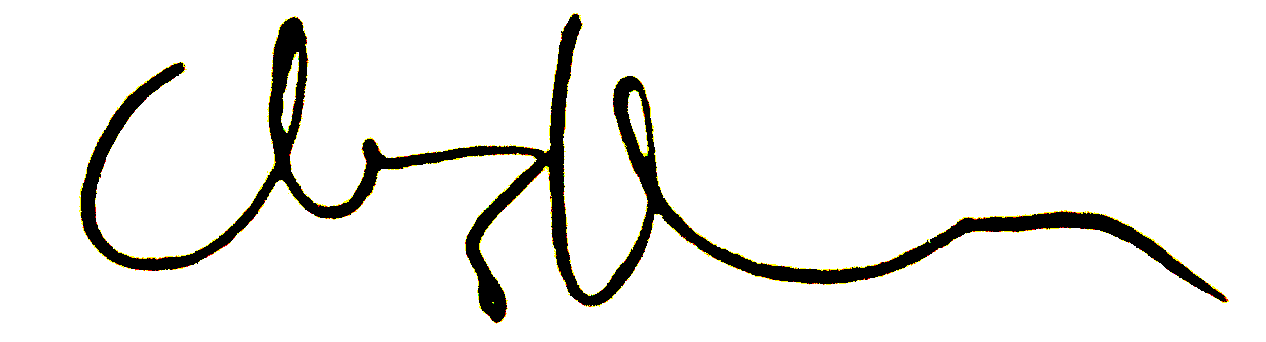
\includegraphics[scale=0.1]{submission/cjb}}\\
Christopher Billington

\vspace{1.5cm}
\rule{8cm}{1pt}\\
\raisebox{0.5cm}[0pt][0pt]{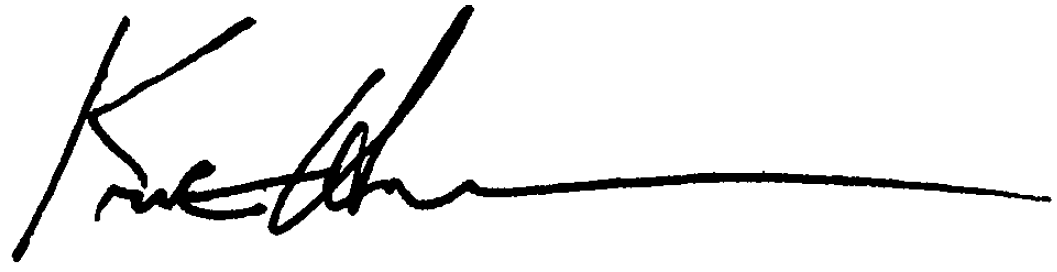
\includegraphics[scale=0.15]{submission/kh}}\\
Professor Kristian Helmerson  

\vspace{1.5cm}
\rule{8cm}{1pt}\\
\raisebox{0.6cm}[0pt][0pt]{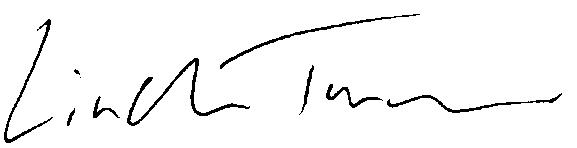
\includegraphics[scale=0.9]{submission/ldt}}\\
Dr Lincoln Turner

\vspace{1.5cm}
\rule{8cm}{1pt}\\
\raisebox{0.5cm}[0pt][0pt]{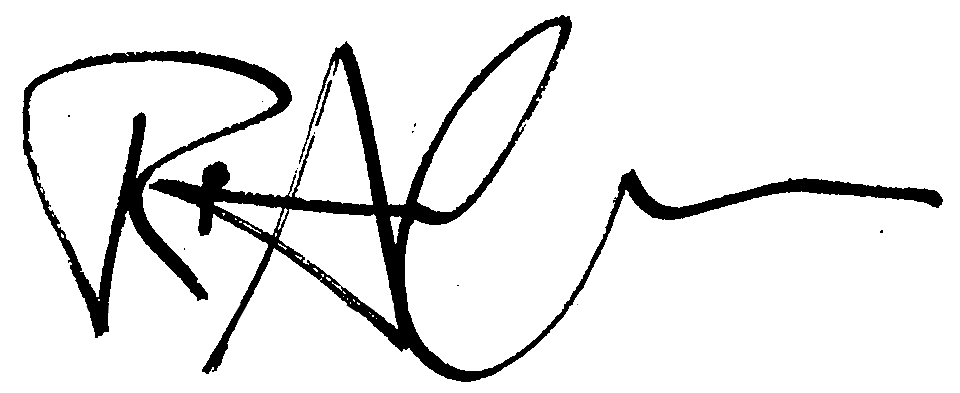
\includegraphics[scale=0.1]{submission/rpa}}\\
Dr Russell Anderson 

\end{center}

\chapter*{Acknowledgements}

Over the past few years during my PhD, I've been able to learn fascinating things from interesting people, play with fun technological toys, and contribute meaningfully to scientific progress. I could not have done any of this without the support, friendship, and mentorship of many people. The Science Advanced cohort---Rory, Shaun, Lisa, Phil---have been much help getting through everything in my (our, mostly) decade-long visit to Monash. My supervisors---Russ, Lincoln, and Kris---have taught me many things, allowed me freedom to follow my curiosity, and provided endless help on endless matters, including getting this thesis over the finishing line, for which Russ deserves special credit. Thanks also to my sister Rosey for proof-reading on short notice, and to Ana for picking up the slack and tolerating me while I neglected most things that were not thesis.

\cleardoublepage

\newgeometry{left=2.54cm,bottom=1.5in,right=2.54cm,top=1.5in}
\thispagestyle{empty}
\vspace*{\fill}
\begin{center}\emph{To Grandma}
\end{center}
\vspace{\fill}
\restoregeometry

\cleardoublepage

\tableofcontents
% \listoffigures
% \listoftables
\cleardoublepage
\pagenumbering{arabic}
